% !TeX root = ../main.tex
\chapter{Introduction}
\label{ch:intro}

\section{Explainable AI}
Artificial intelligence is now an indispensable tool which enhances our life quality.
Due to the increasing complexity of state-of-the-art deep learning models, the AI models are often viewed as a "black box" where only the inputs and the predictions are visualized. This leads to the problem of "trusting" the AI without understanding how it works, as can be seen in Figure \ref{fig:accvsexpl}. Thus, it is becoming more and more important to understand why and how a model reached a certain decision. This is expecially important when the safety of people depends by the AI, such as in healthcare and automotive driving \cite{abeloos2022explaining}.
The techniques used to explain the predictions made by the AI and make them more interpretable are referred to as Explainable AI (XAI). The objective of XAI is to eliminate the "black-box" models by explaining its behavior.
It not only enhances security and trustiness for the end-user, but it also helps the developer to improve the model, for example by removing potential biases. In fact, consider an example in which an object detection model has very good performance metrics. If the dataset contained objects with a specific background, e.g a golf ball with grass as background, then it is highly possible that the model is biased. In that case, it could mistakenly detect a golf ball each time there is grass as background. Through XAI, the developer could easily identify this bias and correct it.
The more explainable a model is, the easier it becomes to improve it. 
XAI could solve security problems: adversarial attacks can mislead an object detector to confuse one image with another just by changing some pixels, leading to unintended behaviors. This is particular critical in automoted driving. Those important pixels attributed by the model could be identified by XAI.
In case of accidents, XAI could help identify the cause, thus improving accountability.

\begin{figure}[h]
    \centering
    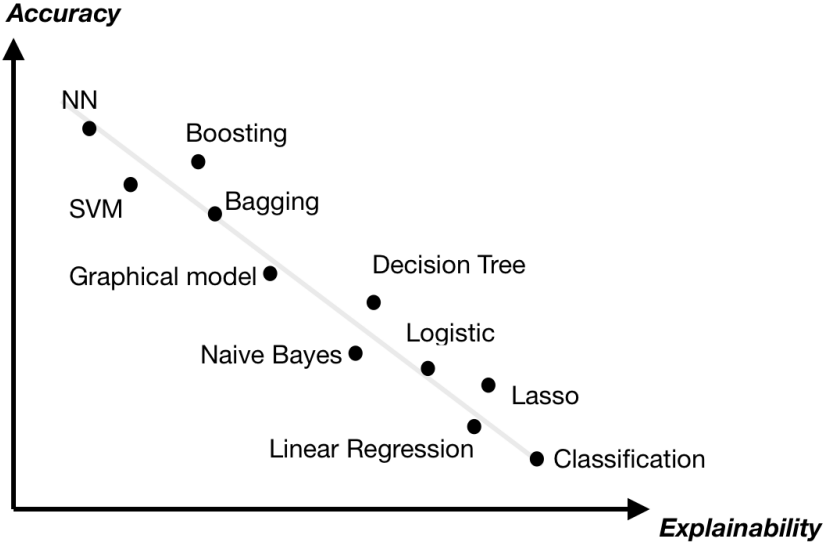
\includegraphics[scale=0.4]{accvsexpl-duval2019explainable}
    \caption{Accuracy vs Explainability of the main machine learning algorithms \cite{duval2019explainable}}
    \label{fig:accvsexpl}
    \end{figure}


\section{Multi-Modal 3D Object Detection}
Autonomous driving is progressing towards self-driving cars thanks to the advanced machine learning models. One of the main difficulties is due to the complex and dynamic driving environment, which require a sofisticated artificial vision \cite{wang2021multi}. Object detection aims to identify the objects in the scene, their location and category \cite{wang2021multi}. Perception with a single modality suffers some drawbacks, such as difficulties on detecting occluded and large objects \cite{huang2022multi}\cite{caesar2020nuscenes}. Equipping the car with more sensors (multi-modal) improves accuracy and robustness. LiDAR (Light Detection and Ranging) sensor contains accurate localization in 3D, while cameras allow measurements of color and edges \cite{caesar2020nuscenes}. It is becoming common to fuse data from LiDAR and cameras for better performance instead of using them separately, but this approach requires precise synchronization.
The success of 2D object detection has been unprecedented thanks to the development of deep learning-based models like RCNN, Fast RCNN, and Faster R-CNN. However, 2D detection can only provide limited information such as the 2D bounding box of an object, which is not enough for autonomous vehicles to perceive their environment. Thus, 3D object detection has become a more challenging but crucial task as it helps with more accurate spatial path planning and navigation. In this task, more output parameters are required to specify the 3D-oriented bounding boxes around objects \cite{wang2021multi}.

% TO-ADD: different types of multi-modal 3D object detection and architectures


\section{Visual Transformers}
%Describe Transformer architecture and its usage in visual applications